\chapter{Brisure de symétrie, bosons de Goldstone et invariance de jauge}

Nous voulons comprendre comment une particule de type photon peut acquérir une masse. C’est le but visé, mais ce n’est pas un point de départ judicieux. Un terme de masse direct pour un champ de jauge semble détruire précisément l’invariance de jauge qui rend la théorie cohérente. Pour trouver une issue, il nous faut d’abord maîtriser deux idées :
\begin{enumerate}
  \item la brisure spontanée de symétrie, en particulier dans le cas d’une symétrie continue ;
  \item l’invariance de jauge, où l’opération de symétrie peut varier d’un point de l’espace-temps à un autre.
\end{enumerate}
Aucune de ces idées ne se réduit à une formule toute faite. Nous allons construire la première à partir d’un aimant, la transposer à la théorie des champs scalaires et découvrir le mode de Goldstone sans masse. Nous rendrons ensuite la même symétrie \(U(1)\) locale, ce qui nous obligera à introduire un potentiel vecteur et une dérivée covariante. Ce n’est qu’à la fin que nous mettrons ces deux fils côte à côte. Leur véritable union---le phénomène de Higgs---fera l’objet du prochain cours.

\section{Une loi symétrique avec un état fondamental asymétrique}

\subsection{L’aimant à deux états}

Partons d’un réseau de petits aimants. Chaque spin peut pointer vers le haut ou vers le bas, et les spins voisins abaissent leur énergie lorsqu’ils pointent dans la même direction. Sur un réseau cubique tridimensionnel, un spin a six plus proches voisins, mais le nombre précis de voisins n’a pas d’importance. Ce qui compte, c’est la règle
\begin{equation}
  E_{\parallel}<E_{\rm antiparallel}.
\end{equation}
La règle microscopique reste inchangée si l’on inverse tous les spins :
\begin{equation}
  \uparrow\longleftrightarrow\downarrow.
\end{equation}
Pourtant, les configurations d’énergie minimale ne sont pas symétriques individuellement. Ce sont
\begin{equation}
  \{\uparrow\uparrow\uparrow\cdots\},
  \qquad
  \{\downarrow\downarrow\downarrow\cdots\}.
\end{equation}
Les équations autorisent les deux, mais un échantillon macroscopique froid doit en choisir une.

Ce choix est d’une sensibilité extraordinaire. Fixons très loin un spin orienté vers le haut. Ses voisins préfèrent s’aligner sur lui, leurs voisins préfèrent s’aligner sur eux, et l’information se propage à travers l’échantillon. Une perturbation arbitrairement faible par rapport au système entier peut sélectionner l’orientation de tout l’état fondamental. C’est cette instabilité que désigne la brisure de symétrie \emph{spontanée}.

\begin{classroomqa}
\audiencequestion{Une particule neutre peut-elle s’orienter dans un champ magnétique ?
\lecturetimestamp{00:05:14}}
\lecturerresponse{Oui. La neutralité électrique n’implique pas l’absence de moment magnétique. Le neutron est neutre, mais il possède un moment magnétique en raison de ses constituants chargés internes. Un champ magnétique peut donc distinguer ses orientations de spin.}
\end{classroomqa}

\begin{classroomqa}
\audiencequestion{Si le système change d’orientation, ce changement se produit-il partout à la fois ? Plusieurs ondes de réorientation peuvent-elles coexister ?
\lecturetimestamp{00:05:41--00:06:38}}
\lecturerresponse{Le changement se propage. Une région fait basculer ses voisines, un peu comme des dominos disposés en trois dimensions, et la perturbation se déplace sous forme d’onde. Des régions différentes peuvent commencer à choisir indépendamment leur orientation ; plusieurs fronts et plusieurs domaines peuvent donc coexister avant que l’une des orientations ne l’emporte. Nous reviendrons précisément sur ces ondes lorsque la symétrie deviendra continue.}
\end{classroomqa}

\subsection{La brisure explicite relève d’une théorie différente}

Plaçons maintenant l’échantillon dans un champ magnétique externe orienté vers le haut. Un spin isolé a déjà une énergie plus faible lorsqu’il pointe vers le haut. La transformation
\(\uparrow\leftrightarrow\downarrow\) ne laisse plus l’énergie inchangée : la préférence a été inscrite dans la loi elle-même. C’est une brisure de symétrie \emph{explicite}.

Cette différence peut être mise à l’épreuve sans connaître la façon dont l’échantillon a été préparé. Prenons un spécimen très grand, imposons une orientation vers le haut à son bord gauche et vers le bas à son bord droit. Si un champ magnétique présent dans le volume favorise explicitement l’orientation vers le haut, la contrainte de droite ne pénètre que sur une faible distance. Une région macroscopique orientée vers le bas aurait un coût énergétique proportionnel à son volume ; le volume ne peut donc pas rester partagé en deux phases également favorables.

En l’absence de champ externe, les orientations vers le haut et vers le bas ont la même énergie dans le volume. L’état contraint d’énergie minimale contient alors un domaine orienté vers le haut, un domaine orienté vers le bas et une couche de transition d’épaisseur finie entre les deux. L’interface n’a pas besoin de se trouver au centre géométrique, mais aucune pression volumique ne force une phase à effacer l’autre. Cette interface est une \emph{paroi de domaine}, le défaut caractéristique de cette symétrie discrète brisée.

\begin{figure}[htbp]
\centering
\begin{adjustbox}{max width=\linewidth}
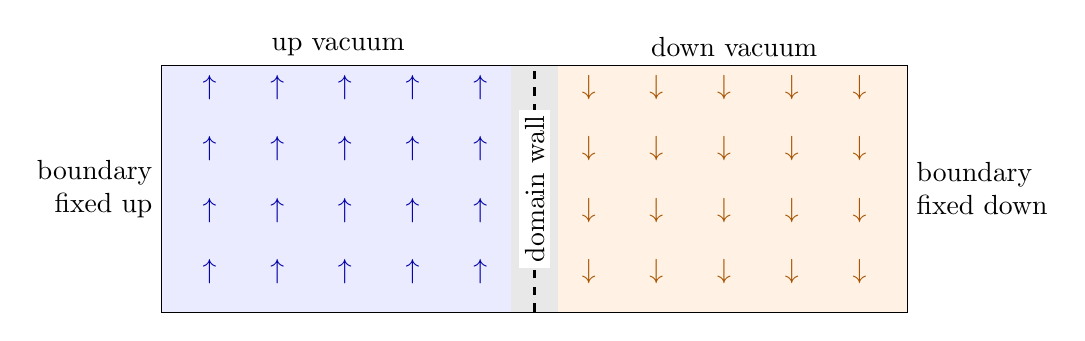
\begin{tikzpicture}[x=0.86cm,y=0.78cm]
  \draw[thick] (0,0) rectangle (11,4);
  \fill[blue!8] (0,0) rectangle (5.15,4);
  \fill[orange!10] (5.85,0) rectangle (11,4);
  \fill[gray!18] (5.15,0) rectangle (5.85,4);
  \foreach \x in {0.7,1.7,2.7,3.7,4.7}
    \foreach \y in {0.65,1.65,2.65,3.65}
      \node[blue!65!black] at (\x,\y) {$\uparrow$};
  \foreach \x in {6.3,7.3,8.3,9.3,10.3}
    \foreach \y in {0.65,1.65,2.65,3.65}
      \node[orange!65!black] at (\x,\y) {$\downarrow$};
  \draw[dashed,thick] (5.5,0) -- (5.5,4);
  \node[above] at (2.6,4) {up vacuum};
  \node[above] at (8.45,4) {down vacuum};
  \node[rotate=90,fill=white,inner sep=2pt] at (5.5,2) {domain wall};
  \node[left,align=right] at (0,2) {boundary\\fixed up};
  \node[right,align=left] at (11,2) {boundary\\fixed down};
\end{tikzpicture}
\end{adjustbox}
\caption{Le test aux frontières pour la brisure spontanée d’une symétrie discrète. Les deux orientations dans le volume ont la même énergie ; une paroi peut donc séparer des domaines macroscopiques.}
\end{figure}

\begin{classroomqa}
\audiencequestion{L’argument exige-t-il que les interactions ne se produisent qu’entre plus proches voisins ?\lecturetimestamp{00:18:18}}
\lecturerresponse{Non. Une interaction entre seconds voisins qui favorise également l’alignement modifie certains détails, mais pas la conclusion. Le comportement devient plus intéressant si les interactions de portées différentes entrent en compétition---les plus proches voisins peuvent, par exemple, préférer l’alignement tandis que les seconds plus proches voisins préfèrent l’anti-alignement. Cela produit de la frustration et des phases ordonnées plus complexes, mais ne change pas la distinction fondamentale établie ici.}
\end{classroomqa}

\begin{classroomqa}
\audiencequestion{Le terme \emph{spontané} désigne-t-il la grande dérivée à l’intérieur de la paroi ?\lecturetimestamp{00:19:05}}
\lecturerresponse{Non. Il désigne le fait que l’énergie sous-jacente ne privilégie aucune orientation haut--bas, alors que l’état fondamental sélectionné, lui, en privilégie une. La réponse spectaculaire à une perturbation arbitrairement faible révèle une instabilité. Le gradient indique simplement le coût de l’interface.}
\end{classroomqa}

\begin{classroomqa}
\audiencequestion{Le matériau se trouvait-il déjà dans l’un des deux états, ou son état était-il initialement inconnu ?\lecturetimestamp{00:19:40}}
\lecturerresponse{Cela dépend de son histoire. À haute température, l’agitation thermique peut maintenir un mélange de spins orientés vers le haut et vers le bas, avec une aimantation moyenne presque nulle. Lorsque le matériau refroidit, des régions choisissent différentes orientations, des parois de domaine se forment, puis les domaines grossissent. Le hasard et de minuscules perturbations de l’environnement déterminent quel vide finit par occuper la plus grande partie de l’échantillon.}
\end{classroomqa}

\section{Le même argument dans la théorie des champs scalaires}

Remplaçons les spins par un champ scalaire réel \(\phi(\bm{x},t)\). Après avoir fixé une fois pour toutes les conventions de métrique et de normalisation, écrivons
\begin{equation}
\begin{aligned}
  \mathcal L
  &=\frac12\,\partial_\mu\phi\,\partial^\mu\phi-V(\phi),
  \\
  \mathcal E
  &=\frac12\dot\phi^{\,2}+\frac12(\nabla\phi)^2+V(\phi).
\end{aligned}
  \label{eq:l07-real-scalar}
\end{equation}
L’écriture relativiste abrégée dans \(\mathcal L\) contient le terme positif de dérivée temporelle et le terme négatif de gradient spatial ; la densité d’énergie hamiltonienne comporte ces deux contributions avec un signe positif.

Choisissons un potentiel pair ayant deux minima dégénérés,
\begin{equation}
  V(\phi)=\frac{\lambda}{4}\left(\phi^2-f^2\right)^2,
  \qquad \lambda>0.
  \label{eq:l07-double-well}
\end{equation}
Le lagrangien est invariant sous \(\phi\mapsto-\phi\), tandis que chacun des deux vides uniformes
\begin{equation}
  \phi(\bm{x})=+f,
  \qquad\hbox{or}\qquad
  \phi(\bm{x})=-f
\end{equation}
en choisit un côté. Un potentiel ayant un minimum unique en \(\phi=0\), en revanche, possède un vide symétrique et ne brise pas spontanément la symétrie.

Fixons \(\phi=+f\) d’un côté de l’échantillon et \(\phi=-f\) de l’autre. Le champ ne peut pas sauter sans coût, car
\begin{equation}
  E_{\rm wall}
  =\int dx\left[
      \frac12\left(\frac{d\phi}{dx}\right)^2+V(\phi)-V(f)
    \right].
  \label{eq:l07-wall-energy}
\end{equation}
Un saut abrupt rend \(d\phi/dx\) énorme. La paroi d’énergie minimale étale donc le changement sur une largeur finie, en équilibrant l’énergie du gradient et le coût potentiel du passage entre les minima. La solution en kink bien connue pour le potentiel de l’équation~\eqref{eq:l07-double-well} est
\begin{equation}
  \phi_{\rm wall}(x)
  =f\tanh\!\left[f\sqrt{\frac{\lambda}{2}}\,(x-x_0)\right],
  \label{eq:l07-kink}
\end{equation}
elle réalise explicitement la transition lisse décrite au tableau.
\editorialnote{L’argument du cours s’appuie sur la forme du potentiel et le terme de gradient, sans résoudre l’équation du champ. L’équation \eqref{eq:l07-kink}est incluse comme solution standard de ce modèle, afin de concrétiser la paroi décrite qualitativement sans modifier l’argument.}

Incliner légèrement le double puits abaisse l’un des minima. Le lagrangien lui-même devient alors asymétrique. Une paroi peut encore apparaître temporairement, mais le faux vide, de plus haute énergie, exerce une pression sur elle ; la paroi se déplace et la phase favorisée s’étend. C’est la version en théorie des champs de la brisure explicite produite par un champ magnétique externe.

Jusqu’ici, la symétrie était discrète. La physique des particules est dominée par des groupes continus tels que \(U(1)\), \(SU(2)\) et \(SU(3)\). Une symétrie continue modifie l’histoire des défauts et fait intervenir une nouvelle sorte de particule.

\section{Un champ complexe et la symétrie globale \texorpdfstring{\(U(1)\)}{U(1)}}

\subsection{Rotations dans un plan interne}

Posons
\begin{equation}
  \phi=\phi_R+i\phi_I,
  \qquad
  \phi^*=\phi_R-i\phi_I,
  \qquad
  \phi^*\phi=\phi_R^2+\phi_I^2.
  \label{eq:l07-components}
\end{equation}
Les axes \(\phi_R\) et \(\phi_I\) forment un espace interne des champs, et non deux directions de l’espace ordinaire. Un champ scalaire complexe est simplement constitué de deux champs scalaires réels regroupés de façon à rendre manifestes les rotations dans ce plan interne.

\begin{figure}[htbp]
\centering
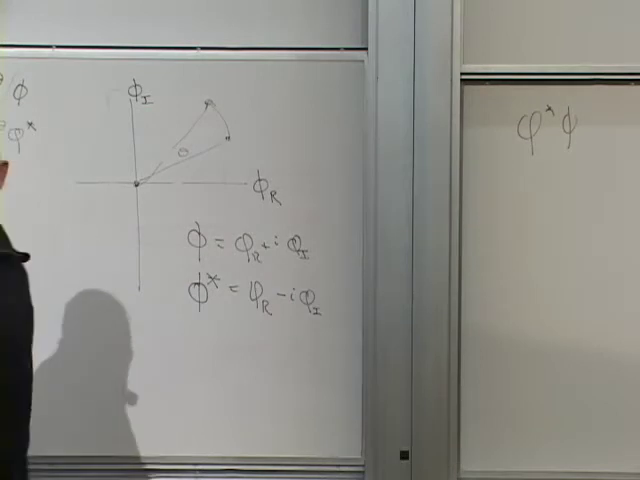
\includegraphics[width=0.80\textwidth]{lecture_07_figure_02.png}
\caption{Le champ complexe dans le plan interne \((\phi_R,\phi_I)\). Le tableau présente la décomposition de \(\phi\) et \(\phi^*\), ainsi que le rayon invariant \(\phi^*\phi\).}
\lectureframe{00:33:33}
\end{figure}

Considérons le lagrangien
\begin{equation}
  \mathcal L
  =\partial_\mu\phi^*\,\partial^\mu\phi
   -V(\phi^*\phi).
  \label{eq:l07-complex-lagrangian}
\end{equation}
Pour un champ complexe, le facteur conventionnel \(1/2\) est absent, car ce produit unique contient déjà les termes cinétiques des deux composantes réelles. La transformation
\begin{equation}
  \phi'(x)=e^{i\theta}\phi(x),
  \qquad
  \phi^{*\prime}(x)=e^{-i\theta}\phi^*(x)
  \label{eq:l07-global-u1}
\end{equation}
fait tourner toutes les valeurs du champ du même angle. Ici, \(\theta\) est constant dans l’espace et le temps. L’apostrophe désigne le champ transformé ; ce n’est pas une dérivée.

Comme \(\theta\) est constant,
\begin{equation}
  \partial_\mu\phi'=e^{i\theta}\partial_\mu\phi,
  \qquad
  \partial_\mu\phi^{*\prime}
  =e^{-i\theta}\partial_\mu\phi^*.
\end{equation}
Les phases s’annulent dans le terme cinétique, et
\(\phi^{*\prime}\phi'=\phi^*\phi\). Ainsi, tout potentiel qui ne dépend que de \(\phi^*\phi\) possède la même symétrie. Un terme dépendant seulement de \(\phi_R\) sélectionnerait une direction dans le plan interne et briserait explicitement cette symétrie.

\subsection{Un minimum ponctuel et un cercle de minima}

Il existe deux types de potentiels symétriques, qualitativement différents. Le premier n’a qu’un seul minimum, à l’origine ; par exemple,
\begin{equation}
  V_{\rm unbroken}=m^2\phi^*\phi,
  \qquad m^2>0.
\end{equation}
Son graphe est un paraboloïde de révolution. Le vide \(\phi=0\)reste inchangé sous toute rotation : la symétrie n’est donc pas brisée.

Choisissons maintenant
\begin{equation}
  V_{\rm broken}
  =-a\,\phi^*\phi+b(\phi^*\phi)^2,
  \qquad a,b>0.
  \label{eq:l07-mexican-hat}
\end{equation}
Le terme quadratique négatif éloigne le champ de l’origine, tandis que le terme quartique positif l’empêche de diverger à l’infini. En posant \(r^2=\phi^*\phi\), la minimisation donne
\begin{equation}
  \frac{dV}{d(r^2)}=-a+2br^2=0,
  \qquad
  r^2=f^2=\frac{a}{2b}.
  \label{eq:l07-vacuum-radius}
\end{equation}
Les minima forment donc un cercle. Le potentiel est parfaitement symétrique par rotation, et pourtant un état fondamental uniforme doit choisir un point de ce cercle.

\begin{figure}[htbp]
\centering
\includegraphics[width=0.72\textwidth]{lecture_07_figure_06.png}
\caption{Le potentiel avec brisure de symétrie, représenté comme une surface de révolution. L’origine est instable et les minima dégénérés forment le creux circulaire.}
\lectureframe{00:37:25}
\end{figure}

Imaginons qu’en chaque point de l’espace ordinaire, le champ soit une petite flèche dans ce plan interne. Le potentiel impose à chaque flèche une longueur \(f\). L’énergie du gradient impose aux flèches voisines de pointer dans des directions presque identiques. L’état fondamental a donc le même angle partout, mais la loi ne privilégie aucun angle. C’est la brisure spontanée d’une symétrie continue.

\section{De la paroi de domaine à la torsion lisse}

Reprenons l’expérience aux frontières. Fixons le champ au bord gauche en un point du vide \(A\) et au bord droit en un autre point du vide \(B\). Un saut localisé rendrait le gradient important. Toutefois, contrairement au cas discret, le champ peut rester au fond du potentiel tout en variant continûment le long du cercle.

À basse énergie, écrivons le champ sous la forme \(\phi=f e^{i\alpha(x)}\). Dans une dimension spatiale, l’énergie pertinente est
\begin{equation}
  E[\alpha]
  =f^2\int_0^L dx\,\left(\frac{d\alpha}{dx}\right)^2.
  \label{eq:l07-angle-functional}
\end{equation}
Pour des angles d’extrémité fixés, la variation donne
\begin{equation}
  \frac{d^2\alpha}{dx^2}=0,
  \qquad
  \alpha(x)=\alpha_A+
    \frac{\alpha_B-\alpha_A}{L}\,x.
  \label{eq:l07-linear-twist}
\end{equation}
La configuration privilégiée répartit uniformément la torsion sur toute la longueur de l’échantillon. Son énergie est proportionnelle à
\begin{equation}
  E_{\rm twist}
  =f^2\frac{(\alpha_B-\alpha_A)^2}{L},
  \label{eq:l07-twist-energy}
\end{equation}
elle peut donc être rendue arbitrairement faible en augmentant \(L\).

\begin{figure}[htbp]
\centering
\begin{adjustbox}{max width=\linewidth}
\begin{tikzpicture}[x=0.95cm,y=0.95cm]
  \begin{scope}
    \draw[->] (0,0) -- (6.2,0) node[right] {$x$};
    \draw[->] (0,0) -- (0,3.5) node[above] {$\alpha(x)$};
    \draw[very thick,blue!70!black] (0.45,0.65) -- (5.7,2.85);
    \fill (0.45,0.65) circle (1.8pt) node[left] {$\alpha_A$};
    \fill (5.7,2.85) circle (1.8pt) node[right] {$\alpha_B$};
    \node at (3.1,-0.65) {physical space};
  \end{scope}
  \begin{scope}[xshift=9.2cm,yshift=1.65cm]
    \draw[thick] (0,0) circle (1.8);
    \fill (1.55,-0.92) circle (1.8pt) node[below right] {$A$};
    \fill (-0.45,1.74) circle (1.8pt) node[above] {$B$};
    \draw[very thick,blue!70!black,-{Latex[length=2.5mm]}]
      (1.55,-0.92) arc[start angle=-31,end angle=104,radius=1.8];
    \node at (0,-2.35) {vacuum circle};
  \end{scope}
\end{tikzpicture}
\end{adjustbox}
\caption{La même configuration de basse énergie représentée de deux façons. L’angle varie linéairement dans l’espace physique, tandis que le champ suit le petit arc du cercle des vides dans l’espace interne.}
\end{figure}

\begin{classroomqa}
\audiencequestion{Il existe deux chemins pour faire le tour du cercle. Lequel le champ emprunte-t-il, et peut-il rester piégé sur le chemin le plus long ?
\lecturetimestamp{00:41:54}}
\lecturerresponse{Pour des extrémités génériques, le chemin angulaire le plus court présente le gradient le plus faible et donc l’énergie la plus basse. Pour des extrémités diamétralement opposées, les deux chemins les plus simples sont dégénérés. Une configuration préparée en déplaçant lentement une extrémité peut conserver un enroulement supplémentaire et rester piégée derrière une barrière d’énergie ; cependant, pour une paire donnée d’extrémités ordinaires, le chemin le plus court, sans torsion, correspond à l’état fondamental.}
\end{classroomqa}

\begin{classroomqa}
\audiencequestion{Le chemin pourrait-il quitter le fond du creux et couper à travers l’intérieur, pour être plus court au total ?
\lecturetimestamp{00:43:32}}
\lecturerresponse{Dans le régime de basse énergie et de grande longueur d’échantillon, il n’est pas avantageux de remonter le potentiel radial. Comme le montre le calcul des variations ci-dessus, le fait de garder le rayon à sa valeur dans le vide et de faire varier linéairement l’angle minimise l’énergie effective. Pour un système fini doté d’un potentiel donné, on peut minimiser ensemble les mouvements radial et angulaire ; mais la conclusion de Goldstone porte sur la limite des longueurs d’onde arbitrairement grandes, où le mouvement lisse le long du creux l’emporte.}
\end{classroomqa}

\begin{classroomqa}
\audiencequestion{Que se passe-t-il si le creux circulaire est incliné, de sorte qu’un angle soit plus bas que les autres ?
\lecturetimestamp{00:44:33}}
\lecturerresponse{La symétrie est alors brisée explicitement. Un point devient le véritable état fondamental, le mouvement le long du cercle acquiert une force de rappel et l’excitation angulaire n’est plus exactement sans masse.}
\end{classroomqa}

\section{La masse comme coût d’une oscillation à impulsion nulle}

La torsion lisse révèle un champ dont l’énergie provient uniquement des gradients. Pour comprendre pourquoi cela signifie qu’une particule est sans masse, comparons la relation de dispersion relativiste
\begin{equation}
  \omega^2=\bm{k}^2+m^2.
  \label{eq:l07-dispersion}
\end{equation}
Une onde \(e^{i(\bm{k}\cdot\bm{x}-\omega t)}\) porte une impulsion \(\bm{k}\). Si \(m=0\), son énergie tend vers zéro lorsque la longueur d’onde tend vers l’infini : \(\omega=|\bm{k}|\to0\). Si \(m\ne0\), un mode spatialement homogène \(\bm{k}=0\) continue d’osciller à la fréquence \(\omega=m\). La masse est l’énergie irréductible à impulsion nulle.

Cette même distinction apparaît dans le lagrangien. Un terme
\begin{equation}
  -\frac12m^2\varphi^2
\end{equation}
fournit une force de rappel même pour un déplacement homogène. Un champ qui ne comporte que des termes dérivés n’a pas de force de rappel de ce type : plus sa longueur d’onde augmente, plus son énergie de gradient tend vers zéro.

\subsection{Les variables polaires séparent les deux modes}

Écrivons le champ complexe avec brisure de symétrie sous la forme
\begin{equation}
  \phi(x)=\rho(x)e^{i\alpha(x)}.
  \label{eq:l07-polar}
\end{equation}
\(\rho\) et \(\alpha\) sont tous deux des champs. En dérivant, on obtient
\begin{align}
  \partial_\mu\phi
  &=e^{i\alpha}
    \left(\partial_\mu\rho+i\rho\,\partial_\mu\alpha\right),\\
  \partial_\mu\phi^*
  &=e^{-i\alpha}
    \left(\partial_\mu\rho-i\rho\,\partial_\mu\alpha\right).
\end{align}
Les termes croisés s’annulent, ce qui laisse
\begin{equation}
  \partial_\mu\phi^*\,\partial^\mu\phi
  =(\partial_\mu\rho)(\partial^\mu\rho)
   +\rho^2(\partial_\mu\alpha)(\partial^\mu\alpha).
  \label{eq:l07-polar-kinetic}
\end{equation}
Puisque \(\phi^*\phi=\rho^2\),
\begin{equation}
  \mathcal L
  =(\partial\rho)^2+\rho^2(\partial\alpha)^2-V(\rho^2).
  \label{eq:l07-polar-lagrangian}
\end{equation}
Le potentiel dépend de \(\rho\), mais pas de \(\alpha\). Cette absence exprime la symétrie sous la forme la plus utile.

\begin{figure}[htbp]
\centering
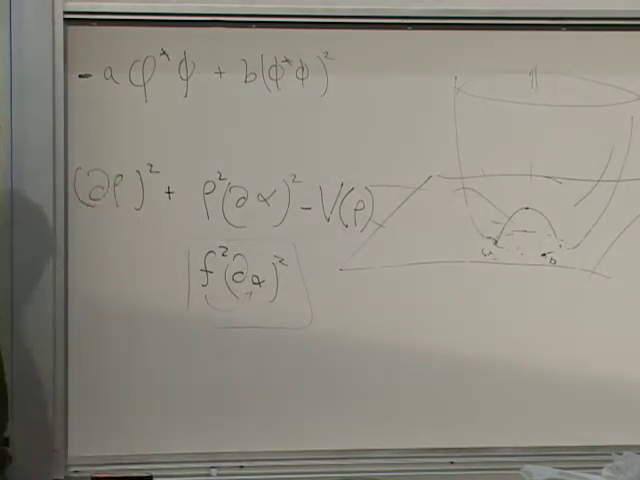
\includegraphics[width=0.88\textwidth]{lecture_07_figure_03.png}
\caption{Le lagrangien en variables polaires, son terme angulaire de basse énergie encadré et le potentiel avec brisure de symétrie. Le mouvement radial remonte le potentiel ; le mouvement angulaire suit le creux.}
\lectureframe{00:56:40}
\end{figure}

Pour une excitation de très basse énergie, le champ reste proche de \(\rho=f\). Alors,
\begin{equation}
  \mathcal L_{\rm angular}
  \simeq f^2(\partial_\mu\alpha)(\partial^\mu\alpha).
\end{equation}
Définissons le champ angulaire normalisé canoniquement, à la convention près pour les facteurs de \(1/2\), par
\begin{equation}
  \beta=\sqrt{2}\,f\alpha,
  \qquad
  \mathcal L_{\rm angular}
  =\frac12(\partial_\mu\beta)(\partial^\mu\beta).
  \label{eq:l07-goldstone-field}
\end{equation}
Il n’y a pas de terme en \(\beta^2\). Les quanta de ce champ angulaire sont sans masse. Ce sont les bosons de Goldstone.

Le champ radial se comporte différemment. Si l’on déplace \(\rho\) par rapport à \(f\) partout à la fois, il retombe, dépasse sa position d’équilibre et oscille autour du creux. Si \(\rho=f+h\), le développement de l’équation~\eqref{eq:l07-mexican-hat} donne
\begin{equation}
  V(f+h)=V(f)+\frac12m_h^2h^2+\cdots,
\end{equation}
\(h\)est donc massif. Géométriquement, la direction angulaire est plate et la direction radiale est courbe.

\begin{classroomqa}
\audiencequestion{Si le champ est déplacé radialement, retombe-t-il simplement, et que se passe-t-il ensuite ?\lecturetimestamp{00:57:10}}
\lecturerresponse{En l’absence de mouvement angulaire, il tombe vers le minimum, le dépasse et oscille radialement. Une oscillation homogène a une impulsion spatiale nulle, mais une fréquence non nulle ; cette fréquence est la masse de l’excitation radiale. En revanche, un déplacement angulaire homogène aboutit à un autre vide et ne subit aucune force de rappel.}
\end{classroomqa}

Dans le présent exemple, le principe de Goldstone affirme donc que la brisure spontanée d’une symétrie globale continue produit un mode sans masse pour chaque direction plate indépendante de la variété des vides.
\editorialnote{Cette affirmation suppose les conditions usuelles de la théorie relativiste des champs. Dans les systèmes à plusieurs corps non relativistes, le dénombrement et la dispersion des modes de Nambu--Goldstone peuvent être plus subtils, mais la conclusion du cours concernant les grandes longueurs d’onde reste valable pour ce modèle relativiste \(U(1)\).}

\section{Ondes de spin, cordes et son}

Le théorème est abstrait, mais son mécanisme est familier. Dans un ferromagnétique isotrope, tous les spins peuvent tourner ensemble sans modifier l’énergie. Si l’orientation varie très lentement à travers l’échantillon, on obtient une onde de spin. Son coût s’annule lorsque son nombre d’onde tend vers zéro : c’est donc le mode de Goldstone associé à la brisure de la symétrie par rotation des spins.

Une longue corde élastique fournit une autre image. Négligeons la gravité et fixons ses extrémités de sorte que toute la corde puisse être translatée verticalement. Une translation verticale uniforme ne coûte aucune énergie. Si cette translation varie lentement le long de la corde, elle devient une onde transverse de grande longueur d’onde. L’opération de symétrie uniforme a été étendue en une déformation douce qui dépend de la position.

\begin{figure}[htbp]
\centering
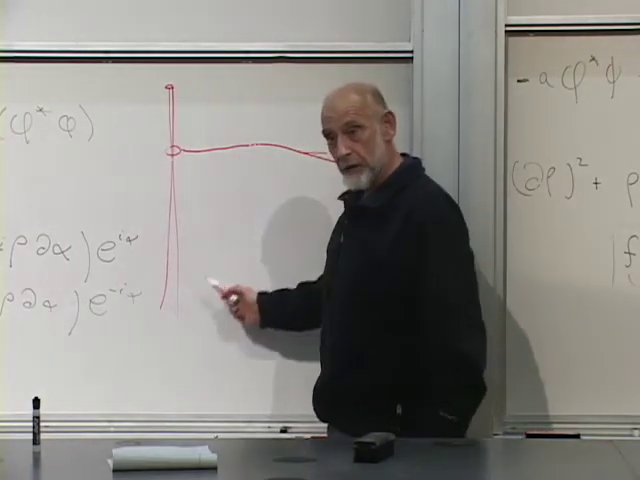
\includegraphics[width=0.68\textwidth]{lecture_07_figure_04.png}
\caption{Le profil de corde lentement variable dessiné pour illustrer l’analogie avec le mode de Goldstone. L’idée physique tient à la faible pente d’une déformation de grande longueur d’onde, et non à la position verticale de la courbe.}
\lectureframe{01:04:19}
\end{figure}

\begin{classroomqa}
\audiencequestion{La corde peut-elle porter une énergie d’oscillation tout en ayant une impulsion nulle ?
\lecturetimestamp{01:04:41}}
\lecturerresponse{Il faut distinguer l’impulsion mécanique verticale de l’impulsion de l’onde le long de la corde. Une onde stationnaire peut avoir une impulsion nette nulle, car elle est une superposition de modes de nombre d’onde \(+k\) et \(-k\), tout en portant de l’énergie. Dans l’analogie avec la théorie des champs, l’impulsion correspond au nombre d’onde le long de l’axe ; le déplacement vertical représente la coordonnée du champ interne.}
\end{classroomqa}

Un ressort hélicoïdal fournit la version longitudinale. Translatons tout le ressort idéal, supposé infini, le long de son axe : rien ne change. Si l’on translate ses parties voisines de quantités légèrement différentes, on obtient une onde de compression douce. Dans un solide ou un fluide, le son de grande longueur d’onde provient de la même façon des déplacements collectifs et des variations de densité. Les ondes de spin, les ondes transverses sur une corde et le son ne sont pas la même excitation microscopique, mais elles partagent le motif décisif : une opération continue uniforme ne coûte aucune énergie, et sa version lentement variable devient un mode mou.
\editorialnote{Dans un cristal, on décrit conventionnellement les phonons acoustiques comme des modes de Nambu--Goldstone associés à la brisure spontanée des translations continues. La corde et le ressort hélicoïdal sont des analogies mécaniques utilisées dans le cours pour mettre en évidence la même structure d’énergie réduite aux termes dérivés.}

La terminologie mérite une brève plaisanterie de cours : ce sont des bosons de \emph{Goldstone}, nommés d’après Jeffrey Goldstone, et non des bosons de jauge. Le cours précise que Goldstone était un ami de Susskind, puis passe au sujet véritablement différent de l’invariance de jauge.

\section{De la symétrie de phase globale à la symétrie de jauge}

La symétrie de phase \(U(1)\) est déjà apparue dans le cours comme la symétrie associée à la conservation de la charge. Les champs des particules chargées sont complexes, et la multiplication d’un tel champ par une phase commune laisse la théorie globale inchangée. On peut parler de charge électrique pour se représenter la situation, même si la charge peut correspondre à un autre nombre quantique \(U(1)\). Le photon réel est sans masse ; le but ultime est un champ de type photon, tel que le \(Z\) massif.

La nouvelle question est de savoir si
\begin{equation}
  \phi'(x)=e^{i\theta(x)}\phi(x)
  \label{eq:l07-local-u1}
\end{equation}
peut être une symétrie lorsque \(\theta\) varie arbitrairement dans l’espace-temps. La fonction \(\theta(x)\) est un paramètre de transformation, et non un champ dynamique supplémentaire. Vérifions cette possibilité en dérivant :
\begin{equation}
  \partial_\mu\phi'
  =e^{i\theta}
   \left[\partial_\mu\phi+i(\partial_\mu\theta)\phi\right].
  \label{eq:l07-local-derivative}
\end{equation}
Le terme supplémentaire était absent lorsque \(\theta\) était constant. Pour le champ conjugué,
\begin{equation}
  \partial_\mu\phi^{*\prime}
  =e^{-i\theta}
   \left[\partial_\mu\phi^*-i(\partial_\mu\theta)\phi^*\right].
\end{equation}
Le produit des deux donne
\begin{align}
  \partial_\mu\phi^{*\prime}\partial^\mu\phi'
  ={}&
  \partial_\mu\phi^*\partial^\mu\phi
  i\left(
      \phi\,\partial_\mu\phi^*
      -\phi^*\partial_\mu\phi
    \right)\partial^\mu\theta
  \nonumber\\
  &+\phi^*\phi\,
    \partial_\mu\theta\,\partial^\mu\theta.
  \label{eq:l07-local-failure}
\end{align}
Le potentiel reste invariant puisque \(\phi^*\phi\), mais le terme cinétique ordinaire ne l’est pas. Une symétrie globale ne devient pas automatiquement une symétrie locale.

\begin{classroomqa}
\audiencequestion{Dans l’image du chapeau mexicain, cet échec signifie-t-il qu’il y a des bosses autour du creux circulaire ?
\lecturetimestamp{01:19:37}}
\lecturerresponse{Non. Le potentiel peut rester parfaitement plat dans la direction angulaire. Le coût supplémentaire provient des gradients lorsque la phase diffère d’un point de l’espace-temps à un autre. Il ne s’agit pas d’une ondulation du creux : c’est le terme de dérivée ordinaire qui détecte la variation spatiale.}
\end{classroomqa}

\subsection{Le champ vectoriel compensateur}

Les interactions du photon naturel, des bosons \(W\), \(Z\) et des gluons s’organisent selon des symétries de jauge locales, et non de simples transformations rigides. Pour que l’opération de phase locale soit une symétrie, élargissons la théorie en y ajoutant un champ quadrivectoriel \(A_\mu\). En électromagnétisme, \(A_0\) est le potentiel scalaire, et les trois composantes spatiales forment le potentiel vecteur. Leurs dérivées construisent les champs électrique et magnétique.

Choisissons la convention cohérente en interne
\begin{equation}
  \phi'=e^{i\theta}\phi,
  \qquad
  A'_\mu=A_\mu-\partial_\mu\theta,
  \qquad
  D_\mu=\partial_\mu+iA_\mu.
  \label{eq:l07-gauge-convention}
\end{equation}
Au tableau, un signe change lors de la vérification de l’annulation ; l’équation \eqref{eq:l07-gauge-convention} fixe conjointement les trois signes. La constante de couplage et la charge sont provisoirement absorbées dans \(A_\mu\).
\editorialnote{En faisant apparaître explicitement la charge \(q\) et la constante de couplage \(g\), on peut écrire \(D_\mu=\partial_\mu+igqA_\mu\) et \(A'_\mu=A_\mu-(gq)^{-1}\partial_\mu\theta\). Le cours supprime ces constantes afin de rendre visible l’annulation.}

Pour le champ conjugué,
\begin{equation}
  D_\mu\phi^*=\partial_\mu\phi^*-iA_\mu\phi^*.
\end{equation}
On a alors
\begin{align}
  D'_\mu\phi'
  &=
  \left(\partial_\mu+iA'_\mu\right)e^{i\theta}\phi
  \nonumber\\
  &=
  e^{i\theta}
  \left[
    \partial_\mu\phi+i(\partial_\mu\theta)\phi
    +i(A_\mu-\partial_\mu\theta)\phi
  \right]
  \nonumber\\
  &=e^{i\theta}D_\mu\phi.
  \label{eq:l07-covariant-transform}
\end{align}
La dérivée indésirable de \(\theta\) est annulée par la transformation de \(A_\mu\). De même,
\begin{equation}
  D'_\mu\phi^{*\prime}=e^{-i\theta}D_\mu\phi^*.
\end{equation}
Leur produit est invariant. L’adjectif \emph{covariant} signifie que la dérivée se transforme aussi simplement que le champ lui-même.

\section{Dynamique du champ de jauge}

Introduire \(A_\mu\) uniquement pour corriger une dérivée laisserait ce champ dépourvu de dynamique propre. Le tenseur de champ, invariant de jauge, est
\begin{equation}
  F_{\mu\nu}
  =\partial_\mu A_\nu-\partial_\nu A_\mu.
  \label{eq:l07-field-strength}
\end{equation}
Il est antisymétrique, donc \(F_{\mu\mu}=0\). Ses composantes temporelles--spatiales contiennent le champ électrique, tandis que ses composantes spatiales--spatiales contiennent le champ magnétique. Dans le langage familier des vecteurs tridimensionnels, la densité d’énergie électromagnétique est proportionnelle à \(\bm E^2+\bm B^2\), tandis que le lagrangien lorentzien est proportionnel à \(\bm E^2-\bm B^2\), les signes dépendant de la convention de métrique.

\begin{classroomqa}
\audiencequestion{Quelles sont l’énergie et le lagrangien du champ électromagnétique ?\lecturetimestamp{01:33:20}}
\lecturerresponse{L’énergie est construite à partir de \(E^2+B^2\) ; le lagrangien utilise \(E^2-B^2\). De manière covariante, ce dernier s’écrit comme un multiple conventionnel de \(F_{\mu\nu}F^{\mu\nu}\). Le tenseur antisymétrique est le rotationnel quadridimensionnel du potentiel vecteur.}
\end{classroomqa}

Le tenseur de champ est lui-même invariant de jauge :
\begin{align}
  F'_{\mu\nu}
  &=
  \partial_\mu(A_\nu-\partial_\nu\theta)
  -\partial_\nu(A_\mu-\partial_\mu\theta)
  \nonumber\\
  &=
  F_{\mu\nu}
  -\partial_\mu\partial_\nu\theta
  +\partial_\nu\partial_\mu\theta
  =F_{\mu\nu}.
  \label{eq:l07-field-strength-invariant}
\end{align}
La dernière égalité découle de la commutation des dérivées partielles mixtes ordinaires. Un lagrangien standard invariant de jauge est donc
\begin{equation}
  \boxed{
  \mathcal L
  =(D_\mu\phi)^*D^\mu\phi
  -V(\phi^*\phi)
  -\frac14F_{\mu\nu}F^{\mu\nu}}
  \label{eq:l07-scalar-qed}
\end{equation}
à un signe et à une normalisation près, selon les conventions de métrique choisies.

\begin{figure}[htbp]
\centering
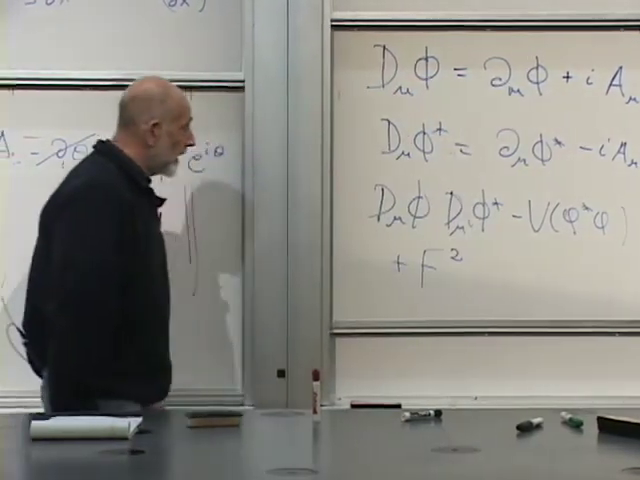
\includegraphics[width=0.84\textwidth]{lecture_07_figure_05.png}
\caption{Les dérivées covariantes et le lagrangien invariant de jauge assemblés au tableau. Les facteurs numériques y sont omis afin de laisser apparaître la structure des transformations.}
\lectureframe{01:38:45}
\end{figure}

Cette construction rend locale une symétrie globale \(U(1)\), mais elle le fait au prix---ou, physiquement, grâce au don---d’un nouveau champ vectoriel. Dans l’exemple abélien, ce champ est le potentiel électromagnétique.

\begin{classroomqa}
\audiencequestion{Le lagrangien de départ utilisait des dérivées ordinaires. Pourquoi sommes-nous autorisés à les remplacer par des dérivées covariantes et à qualifier le résultat de véritable théorie ?\lecturetimestamp{01:42:55}}
\lecturerresponse{Nous construisons une théorie différente et élargie : de la matière chargée associée à un champ de jauge. L’invariance de jauge locale détermine leur couplage. La théorie quantique qui en résulte forme une structure mathématique cohérente et concorde avec la façon dont la nature organise le photon et les champs de jauge faibles. Un couplage incohérent d’un champ vectoriel relativiste peut simplement introduire des polarisations non physiques et des violations de la probabilité ; le principe de jauge n’est donc pas une réécriture cosmétique de l’ancienne théorie du champ scalaire libre.}
\end{classroomqa}

\begin{classroomqa}
\audiencequestion{L’ajout du nouveau champ est donc la justification essentielle de cette modification ?\lecturetimestamp{01:44:57}}
\lecturerresponse{Oui. Sans \(A_\mu\), la dérivée d’un champ tourné localement contient un terme \(\partial_\mu\theta\) qui n’est pas compensé. Avec \(A_\mu\) et sa loi de transformation, la compensation fonctionne. En langage géométrique, \(A_\mu\) est une connexion sur un fibré ; ces mathématiques plus profondes sont bien réelles et utiles, mais le calcul ci-dessus contient tout ce dont nous avons besoin ici.}
\end{classroomqa}

\section{Pourquoi une masse nue pour un boson de jauge est interdite}

Pour un champ bosonique ordinaire, une masse se représente par un terme quadratique. On pourrait être tenté d’ajouter
\begin{equation}
  \Delta\mathcal L_{\rm Proca}
  =\frac12m^2A_\mu A^\mu.
  \label{eq:l07-proca}
\end{equation}
Mais sous la transformation \(A_\mu\mapsto A_\mu-\partial_\mu\theta\),
\begin{equation}
  A'_\mu A^{\mu\prime}
  =
  A_\mu A^\mu
  -2A^\mu\partial_\mu\theta
  +\partial_\mu\theta\,\partial^\mu\theta,
\end{equation}
l’équation~\eqref{eq:l07-proca} n’est donc pas invariante de jauge. Nous ne pouvons pas introduire à la main une masse dans cette théorie de jauge tout en conservant sa symétrie locale.

\begin{figure}[htbp]
\centering
\includegraphics[width=0.72\textwidth]{lecture_07_figure_07.png}
\caption{La masse nue proposée pour le champ vectoriel
\(\tfrac12m^2A_\mu A^\mu\). Son comportement sous la transformation
\(A_\mu\mapsto A_\mu-\partial_\mu\theta\) constitue l’obstacle qui ouvre la voie au mécanisme de Higgs.}
\lectureframe{01:39:48}
\end{figure}

C’est l’impasse apparente. L’invariance de jauge explique la masse nulle du photon et protège la théorie contre les degrés de liberté non physiques, mais les \(W\) et \(Z\) sont massifs. On ne peut pas sortir de cette impasse en introduisant explicitement une masse vectorielle. Il faut que celle-ci résulte des champs déjà présents dans un lagrangien invariant de jauge.

\begin{classroomqa}
\audiencequestion{L’introduction de l’invariance de jauge produit-elle elle-même le boson de Goldstone ?\lecturetimestamp{01:45:51}}
\lecturerresponse{Non. Le boson de Goldstone est apparu lorsqu’une symétrie \emph{globale} continue a été spontanément brisée, avant l’introduction du potentiel vecteur. Une fois la symétrie rendue locale, une phase variable peut être compensée par \(A_\mu\). Dans la théorie de jauge brisée, le mode angulaire n’est plus une particule sans masse indépendante ; il fournit la polarisation supplémentaire du champ vectoriel désormais massif. Le prochain cours établira ce résultat au lieu de se contenter de l’annoncer.}
\end{classroomqa}

\begin{classroomqa}
\audiencequestion{Tout cela explique-t-il pourquoi les rivières forment des méandres ?
\lecturetimestamp{01:47:03}}
\lecturerresponse{Aucun lien direct n’est connu ici. Les tourbillons des fluides et même les formes des organismes peuvent assurément être décrits à l’aide de méthodes fondées sur les symétries, et il ne faut jamais s’étonner de trouver des idées de théorie des champs dans des endroits inattendus, mais le cours ne prétend pas proposer une théorie de jauge des méandres des rivières.}
\end{classroomqa}

\section{Où s’arrête le cours}

Nous disposons maintenant des deux éléments annoncés au début. Une symétrie globale continue dont les vides forment un cercle possède une direction angulaire plate, et ses variations lentes donnent un champ de Goldstone sans masse. Une symétrie locale exige une connexion de jauge et des dérivées covariantes, et interdit la masse vectorielle directe de l’équation~\eqref{eq:l07-proca}.

L’étape suivante consiste à intégrer le potentiel brisé de l’équation~\eqref{eq:l07-mexican-hat} dans la théorie invariante de jauge de l’équation~\eqref{eq:l07-scalar-qed}. Deux choses se produisent alors simultanément : la particule de Goldstone distincte disparaît du spectre physique, et le champ vectoriel acquiert une masse. Dans le langage pédagogique courant, la symétrie de jauge est spontanément brisée ; plus précisément, la redondance de jauge subsiste, tandis que la théorie entre dans une phase de Higgs comportant une excitation vectorielle massive.
\editorialnote{Une symétrie de jauge locale est une redondance de description, et non une symétrie physique ordinaire agissant entre des états observables distincts. Le cours emploie le raccourci courant de la brisure spontanée de la symétrie de jauge. L’énoncé physique invariant de jauge décrit le réarrangement des degrés de liberté dans la phase de Higgs.}

C’est le phénomène de Higgs. Nous ne l’avons pas encore mis en œuvre. Ce cours a accompli le travail préalable, plus difficile, qui consistait à formuler le problème avec assez de précision pour que la solution, lorsqu’elle sera présentée, s’impose.